\part{Geophysical Fluid Dynamics}\label{Geophysical Fluid Dynamics}

\section*{Introduction}

This section of the course was lectured by \href{https://www.physics.ox.ac.uk/our-people/woollings}{Tim Woollings} covering Geophysical Fluid Dynamics.\vspace{5 mm}

\noindent This section consists of three chapters:\vspace{5 mm}

\begin{enumerate}
    \item \hyperref[Dynamical Systems]{Dynamical Systems}: 
        
        \begin{quote}
            Meow
        \end{quote}

    \item \hyperref[Predictability]{Predictability}: 
    
        \begin{quote}
            Meow
        \end{quote}
    
    \item \hyperref[Estimation]{Estimation}:
        
        \begin{quote}
            Meow
        \end{quote}
\end{enumerate}

\chapter{Preliminaries}

\section{A Quick Reminder of Vector Calculus}

Before we jump into \textbf{Geophysical Fluid Dynamics} (\textbf{GFD}) proper, we start with a quick reminder of some concepts in vector calculus. This will be important for the interpretation of certain results.

We work in a 3-dimensional cartesian coordinate system and write the spatial coordinates as $(x,y,z)$ and the spatial unit vectors as $(\hat{i},\hat{j},\hat{k})$. We can write any position vector $\vec{r}$ as $\vec{r}=x\hat{i}+y\hat{j}+z\hat{k}$. For brevity later on, I will often refer to the $i$th coordinate as $x_i$ (i.e., $x=x_1$, $y=x_2$, $z=x_3$).

We will encounter many \textbf{fields} throughout GFD. A \textbf{field} is just anything that has a value at each point in space and time. There are two kinds you will need to know: a \textbf{scalar field} and a \textbf{vector field}. A \textbf{scalar field} is a field that takes a scalar value at each point. For example, the pressure field $p=p(\vec{r},t)$ is a scalar field, which denotes the pressure at each point in space/time. Meanwhile, a \textbf{vector field} is a field that takes a vector value at each point. For example, the velocity field $\vec{u}=\vec{u}(\vec{r},t)$ is a vector field, which denotes the velocity at each point in space/time. While it isn't strictly correct, you can just think of a vector field as three scalar fields stacked on top of each other (one for each component).

All of this section will be devoted to how we calculate derivatives of such fields. Fields are special in the sense that they depend on more than one dimension, so we cannot simply use the good ol' derivative/integral that we know from single variable calculus.

We introduce the partial derivative $\partial/\partial x_i$ with respect to coordinate $x_i$. This is completely analogous to the more familiar derivative, so you can calculate this by simply differentiating with respect to $x_i$ and treating all other coordinates ($x_j$ for $j\neq i$ and $t$) as constant. You can denote the partial derivative 

We also introduce the nabla operator $\vec{\nabla}=\left( \frac{\partial}{\partial x}, \frac{\partial}{\partial y}, \frac{\partial}{\partial z} \right)^T$. This allows as to calculate different things from scalar and vector fields. We define the \textbf{gradient}, \textbf{divergence}, and \textbf{curl}.

The gradient is defined as a vector field calculated by using the nabla operator on a scalar field. We will d

The divergence is defined as a scalar field calculated b

\begin{fact}{Vector Calculus Reminder}{VC box}\label{VC box}
    We define the 
    \begin{align*}
        \frac{\partial}{\partial x_i}
    \end{align*}
    \begin{align*}
        \vec{\nabla}=\left( \frac{\partial}{\partial x}, \frac{\partial}{\partial y}, \frac{\partial}{\partial z} \right)^T
    \end{align*}
\end{fact}



\section{A Quick Reminder of Fluid Mechanics}

To aid understanding, we quickly introduce some concepts of fluid mechanics. Tim should have a more comprehensive review on canvas should you need it.

First we introduce the concept of a fluid element. This is an infinitesimal volume of fluid, whose properties may change as it is advected around with the flow. For example, in deriving the \hyperref[Dry Adiabat]{Dry Adiabat}, we were considering a fluid element of air – except we called it an `air parcel' then.

Second, we introduce the \hyperref[Material Derivative]{Material Derivative}:
\begin{align}
    \frac{D}{Dt}=\underbrace{\frac{\partial}{\partial t}}_{\text{Time Derivative at a Fixed Point}}+\underbrace{\vec{u}\cdot\vec{\nabla}}_{\text{Advection}}
    \label{Material Derivative}
\end{align}
The \hyperref[Material Derivative]{Material Derivative} of a quantity is the time-derivative of a quantity \textit{following a fluid element}. This is useful because it is much easier to consider what effects might change a quantity of a fluid element. For example, the forces per unit mass $\vec{F}$ affect a fluid parcel as follows: $\frac{D\vec{u}}{Dt}=\vec{F}$ (this is just Newton's second law).

However, in GFD, we will mostly be interested in how a quantity changes at a \textbf{fixed point in space} $\left(\text{indicated by the } \frac{\partial}{\partial t} \text{ term}\right)$, \textit{not following a fluid element}. If we rearrange the Equation \ref{Material Derivative} for $\left( \frac{\partial}{\partial t} \right)$, we find that the quantity at some point is modified by both whatever affects the fluid element $\left( \frac{D}{D t} \right)$, for example the force $\vec{F}$, and the properties of fluid elements which are advected into that location $-\vec{u}\cdot\vec{\nabla}$:
\begin{align}\label{MatDerivTerms}
    \underbrace{\frac{\partial A}{\partial t}}_{\text{Local change in }A}=
    \underbrace{\frac{DA}{Dt}}_{{\text{Change in }A \text{ following a fluid element}}}-
    \underbrace{\vec{u}\cdot\vec{\nabla}A}_{\text{Advection of fluid elements with different }A}
\end{align}

Third, we introduce the idea of \hyperref[Material Conservation]{Material Conservation}. You might have heard about what it means for a quantity to be \textbf{conserved}. For example, if you've solved a mechanics problem, you might recall that the total energy was conserved, meaning that $\frac{dE}{dt}=0$ where $E=$ the total energy.

\hyperref[Material Conservation]{Material Conservation} is a closely related idea, where certain quantities are conserved following a fluid parcel. Mathematically, a quantity $A$ is materially conserved if and only if it obeys the following relation:
\begin{align}\label{Material Conservation}
    \frac{D A}{Dt }=0
\end{align}
In other words, if one follows a fluid parcel, that quantity does not change. However, as a whole, $A$, need not be globally conserved. If one considers Equation \ref{MatDerivTerms} and sets $\frac{D A}{Dt }=0$, then you can see that the only local change in $A$ is from fluid parcels with different $A$ being advected into that location.

Exercise: refer forwards to Equation \ref{Energy Equation}. Note even if we assume that $Q=0$, we will find that $\frac{DT}{Dt}\neq 0$. In other words, temperature is not materially conserved (so long as $\beta\neq0$). This is why we introduced the idea of \hyperref[Potential Temperature]{Potential Temperature}, as it is the case that $\frac{D\theta}{Dt}=0$ (excercise: take \ref{Energy Equation}, solve for $\beta$ using the ideal gas law, set $Q=0$, and show that $\frac{D\theta}{Dt}=0$ using the product rule).

\section{Why There Is Motion in the First Place}

It's important to consider why there is motion in the Atmospheres and the Oceans in the first place, and what sets \textbf{Geophysical Fluid Dynamics} apart from most other Fluid Dynamics.

Regarding the first point, if you are familiar with the \hyperref[Navier Stokes]{Navier Stokes Equations} governing fluid flow, then you will know that $\vec{u}=\vec{\nabla}p=0$ is a solution, and is a solution a system will tend towards if there is friction, and planets certainly have plenty of friction. We therefore need a non-uniform energy source. In this case, it is the sun, and it drives motion because it provides energy to the Earth unevenly. On small scales, this may be because of variations in reflectivity (albedo), but on large scales this is mostly due to the spherical geometry of the Earth: more solar radiation is absorbed at the equator than at the poles (think: \textbf{zenith angle} from \hyperref[Radiative Transfer]{Radiative Transfer}, which goes as $\cos\zeta$).

This differential heating causes horizontal temperature gradients, which in turn cause horizontal density and pressure gradients, which drive motion. Another way to think of it is as follows: in equilibrium, the Earth absorbs more solar radiation in the equator than in the poles (see Figure \ref{Diff Heating}). As such, there must be an energy transport mechanism from the equator to the poles, and this is what drives fluid motion.\footnote{
    I'm personally somewhat ambivalent about this explanation, but I'm not very confident so be sceptical of what I'm about to say. Here's why I'm uncomfortable about this explanation: I cannot see why it must be the case that the variation in OLR cannot be identical to the variation in absorbed solar radiation. To put it another way, I cannot see why the dotted curve cannot be identical to the solid curve in Figure \ref{Diff Heating}. The absorbed energy per unit area scales as $\cos\phi$, where $\phi$ is the latitude. It feels like putting the cart before the horse: surely the fluid dynamics also itself affects the OLR into space.
}

\begin{figure}[H]
    \centering
    \includegraphics[width=0.5\linewidth]{Figures/GFD/Diff Heating.jpg}
    \caption{Figure from Ray's book showing differential heating. More heat is }
    \label{Diff Heating}
\end{figure}

\section{What is Special About `Geophysical' Fluid Mechanics?}

Regarding the second point, there are two important properties that separate \textbf{Geophysical Fluid Dynamics} into its own field: that of \textbf{stratification} and \textbf{rotation}. The effects of these will pop up again and again throughout this part.

\textbf{Stratification} is 

\chapter{The Equations of Motion}

\section{The Primitive Equations of Motion}

For simplicity we ignore state variables like salinity, humidity, etc., and restrict our attention to a system fully characterised by 6-state variables: the velocity $\vec{u}=(u,v,w)$, pressure $p$, density $\rho$, and temperature $T$. These are governed by six equations: 3 momentum budget equations (\ref{Navier Stokes}), one mass budget equation (\ref{Mass Conservation}), one energy budget equation (\ref{Energy Equation}), and an equation of state (\ref{EoS}). Each term is labelled below:
\begin{gather}
    \boxed{\underbrace{\frac{D\vec{u}}{Dt}}_{\text{Acceleration and Advection}}
    =\overbrace{-\frac{1}{\rho}\vec{\nabla}p}^\text{Pressure Gradients}\underbrace{-g\vec{k}}_\text{Gravity}+\overbrace{\nu\vec{\nabla}^2\vec{u}}^\text{Viscous Dissipation}\underbrace{+\frac{\nu}{3}\vec{\nabla}(\vec{\nabla}\cdot\vec{u})}_\text{}+\overbrace{\vec{F}}^\text{Other Forces}}
    \label{Navier Stokes}
    \\
    \boxed{\underbrace{\frac{D\rho}{Dt}}_\text{Change in Mass of Fluid Parcel}\overbrace{+\rho\vec{\nabla}\cdot\vec{u}}^\text{Convergence/Divergence of Mass}=0}
    \label{Mass Conservation}
    \\
    \boxed{c_p\frac{DT}{Dt}-\frac{\beta T}{\rho}\frac{Dp}{Dt}=Q}
    \label{Energy Equation}
    \\
    \boxed{\rho=\rho(T,p,\ldots)}
    \label{EoS}
\end{gather}

\noindent where $\frac{D}{Dt}=\frac{\partial}{\partial t}+\vec{u}\cdot\vec{\nabla}$ is the material derivative; $g=$ gravitational acceleration; $\vec{k}=$ unit vector towards the centre of the Earth; $\nu=$ kinematic viscocity; $\vec{F}=$ other forces per unit mass (e.g., friction); $c_p=$ heat capacity per unit mass; $\beta=-\frac{1}{\rho}\frac{\partial \rho}{\partial T}$ thermal expansion coefficient; and $Q=$ heating per unit mass.

However, the equations currently are not fit for purpose. First, these equations are written for a coordinate system that is \textit{inertial} (non-accelerating) and \textit{cartesian}. However, the surface of the Earth is curved and the Earth is rotating\footnote{or so NASA and the lizard overlords would have you think!}, and we wish to describe what is going on \textit{here} with us. Furthermore, it would be quite demanding (computationally and conceptually) to adopt an inertial non-curved coordinate system, as then you'd have to, for example, keep track of the fact that the mountains keep moving. 

Second, these equations are currently too complicated to be analytically tractable. We will make various approximations later to simplify the equations of motion, however we should note that many of the terms we neglect cannot be neglected in a weather forecast or climate model.

\section{Simplifications}

\subsection{Rotating Coordinate Systems}

As already mentioned, the momentum budget equation applies for an \textit{inertial coordinate system}, i.e., a coordinate system which is not accelerating. However we wish to describe the dynamics in a rotating coordinate system which rotates with the Earth (or planet). Our goal now is to  find a relation between the time derivative of some arbitrary vector $\vec{A}$ in an inertial coordinate system $\left(\frac{d\vec{A}}{dt}\right)_I$ and the time derivative in a rotating coordinate system $\left(\frac{d\vec{A}}{dt}\right)$.

We consider two coordinate systems: an \textit{inertial} coordinate system and a \textit{rotating} coordinate system. Both systems share an origin, but the \textit{inertial} coordinate system rotates with a constant angular velocity $\vec{\Omega}$ where $|\vec{\Omega}|$ is the angular speed (in \qty{}{\radian\per\second}) and $\vec{\Omega}$ points along the axis of rotation.

Now consider some arbitrary vector $\vec{A}(t)$ in or rotating coordinate system. The time derivative in the inertial coordinate system $\left(\frac{d\vec{A}}{dt}\right)_I$ is related to the time derivative in the rotating coordinate system $\left(\frac{d\vec{A}}{dt}\right)_R$ as follows (see Figure \ref{Inertial to Rotating}):
\begin{figure}
    \centering
    \begin{subfigure}{0.4\linewidth}
        \centering
        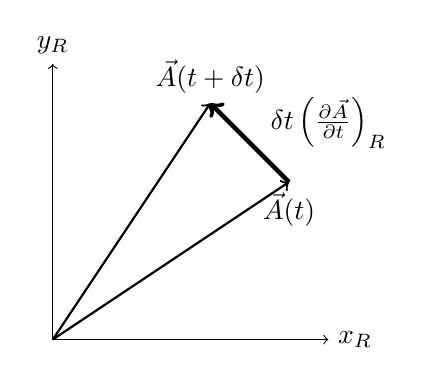
\begin{tikzpicture}
            \draw[->] (0,0) -- (3.5,0) node[anchor=west] {$x_R$};
            \draw[->] (0,0) -- (0,3.5) node[anchor=south] {$y_R$};
            \draw[thick,->] (0,0) -- (3,2) node[anchor= north] {$\vec{A}(t)$};
            \draw[thick,->] (0,0) -- (2,3) node[anchor=south] {$\vec{A}(t+\delta t)$};
            \draw[ultra thick,->] (3,2) -- (2,3) {};
            \node[] at (3.5,2.75) {$\delta t \left( \frac{\partial \vec{A}}{\partial t} \right)_R$};
        \end{tikzpicture}
        \caption{Change in $\vec{A}$ in the Rotating Coordinate System}
        \label{Rotating}
    \end{subfigure}
    \hfill
    \begin{subfigure}{0.4\linewidth}
        \centering
        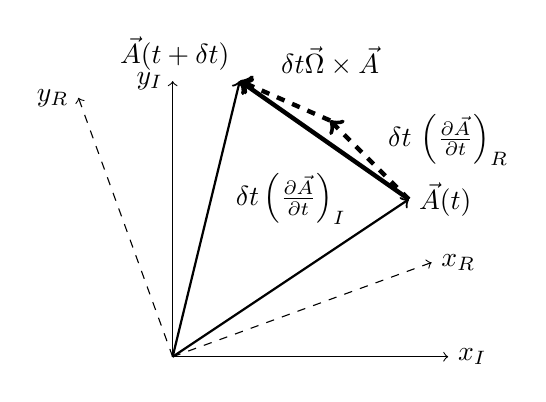
\begin{tikzpicture}
            \draw[->] (0,0) -- (3.5,0) node[anchor=west] {$x_I$};
            \draw[->] (0,0) -- (0,3.5) node[anchor=east] {$y_I$};
            \draw[thick,->] (0,0) -- (3,2) node[anchor=west] {$\vec{A}(t)$};
            %\draw[dotted,->] (0,0) -- (2,3) node[anchor=south] {};
            \draw[thick,->] (0,0) -- (0.853,3.503) node[anchor=south east] {$\vec{A}(t+\delta t)$};
            \draw[ultra thick,->,dashed] (3,2) -- (2,3) {};
            \node[] at (3.5,2.75) {$\delta t \, \left( \frac{\partial \vec{A}}{\partial t} \right)_R$};
            \draw[ultra thick,->,dashed] (2,3) -- (0.853,3.503) {};
            \node[] at (2,3.75) {$\delta t \vec{\Omega}\times\vec{A}$};
            \draw[->,dashed] (0,0) -- (3.289,1.197) node[anchor=west] {$x_R$};
            \draw[->,dashed] (0,0) -- (-1.197,3.289) node[anchor=east] {$y_R$};
            \draw[ultra thick,->] (3,2) -- (0.853,3.503);
            \node[] at (1.5,2) {$\delta t \left( \frac{\partial \vec{A}}{\partial t} \right)_I$};
        \end{tikzpicture}
        \caption{Change in $\vec{A}$ in the Inertial Coordinate System}
        \label{Inertial}
    \end{subfigure}
    \caption{The change in $\vec{A}$ in a rotating (\ref{Rotating}) and inertial (\ref{Inertial}) coordinate system. As seen in \ref{Inertial}, the change in the inertial coordinate system $\delta t \left( \frac{\partial \vec{A}}{\partial t} \right)_I$ (thick arrow) is equal to sum of the change in the rotating coordinate system $\left( \delta t \left( \frac{\partial \vec{A}}{\partial t} \right)_R \right)$ \textit{and} the rotation of the rotating coordinate system $\left(\delta t\,\vec{\Omega}\times\vec{A} \right)$ (thick dashed arrows).}
    \label{Inertial to Rotating}
\end{figure}
\begin{align}
    \left(\frac{d\vec{A}}{dt}\right)_I=\left(\frac{d\vec{A}}{dt}\right)_R+\vec{\Omega}\times\vec{A}
    \label{Rotating Relation}
\end{align}

If we let $\vec{A}=\vec{r}$, where $\vec{r}$ is the position of our fluid parcel, we can apply Equation \ref{Rotating Relation} twice to obtain an expression for the acceleration of a fluid parcel in a rotating coordinate system.
\begin{align*}
    \vec{u}_I &= \left( \frac{d\vec{r}}{dt} \right)_I\\
    &= \left( \frac{d\vec{r}}{dt} \right)_R+\vec{\Omega}\times \vec{r}\\
    \vec{u}_I & = \vec{u}_R+\vec{\Omega}\times \vec{r}\\
    \therefore \vec{a}_I & =
    \left( \frac{d\vec{u}_I}{dt} \right)_I\\
    &= \left( \frac{d\vec{u}_I}{dt} \right)_R+\vec{\Omega}\times \vec{u}_I\\
    &= \left( \frac{d\vec{u}_R}{dt} \right)_R
    +\vec{\Omega}\times\left( \frac{d\vec{r}}{dt} \right)_R
    +\vec{\Omega}\times\left( 
        \vec{u}_R+\vec{\Omega}\times \vec{r}
     \right)\\
    &=\vec{a}_R+2\vec{\Omega}\times\vec{u}_R+\vec{\Omega}\times\vec{\Omega}\times\vec{r}
\end{align*}

Therefore the acceleration in the rotating frame of reference $\vec{a}$ is equal to the acceleration in a inertial coordinate system summed with two fictitious\href{https://xkcd.com/123/}{$^*$}  forces: the \textbf{centrifugal force} and the \textbf{coriolis force}.
\begin{align}
    \vec{a}_R=\vec{a}_I+\underbrace{2\vec{\Omega}\times\vec{u}_R}_\text{Coriolis}
    +\underbrace{\vec{\Omega}\times\vec{\Omega}\times\vec{r}}_\text{Centrifugal}
\end{align}

The \textbf{centrifugal force} is the force that pushes objects away from the axis of rotation. This is the force that makes your arms fling out if you spin. The \textbf{coriolis force} is the force that diverts moving objects which move away or towards the axis of rotation. 

We have thus transformed Equation \ref{Navier Stokes} into a rotating coordinate system:
\begin{align}
    \frac{D\vec{u}}{Dt}+2\vec{\Omega}\times\vec{u}+\frac{1}{\rho}\vec{\nabla}p+g\vec{k}=-\vec{\Omega}\times\vec{\Omega}\times\vec{r}+\nu\vec{\nabla}^2\vec{u}+\frac{\nu}{3}\vec{\nabla}(\vec{\nabla}\cdot\vec{u})+\vec{F}\label{Navier Stokes Rotating}
\end{align}

\subsection{Local Cartesian Coordinates}

We have just learnt how to deal with coordinate systems that vary with time. We will now skim over (since the details aren't that interesting) how to deal with coordinate systems that vary with space.

We wish to use a coordinate system that follows the surface of the Earth, with the basis vectors $\hat{x}$, $\hat{y}$, $\hat{z}$, pointing in the east, north, and upwards (away from the centre of the Earth) directions. In this coordinate system, we define the position and velocity coordiates $(x,y,z)$ and $(u,v,w)$ as indicating distance and velocity in the east, north, and upwards directions, respectively. We further define the latitude $\phi\in[-\frac{\pi}{2},\frac{\pi}{2}]$ ($\phi=0$ indicates the equator, $\phi=\pm\frac{\pi}{2}$ is the north/south pole) and the radial distance $r$ where $r=a+z$ where $a=$ the radius of the Earth (see Figure \ref{LocCartes}).
\begin{figure}[H]
    \centering
    \scalebox{1.4}{
    \begin{tikzpicture},
        \begin{scope}[3d view={125}{25.26}]
            \draw[->,opacity=0.7] (0,0,0) -- (1.5,0,0) node[anchor=north east] {$x'$};
            \draw[->,opacity=0.7] (0,0,0) -- (0,1.5,0) node[anchor=north] {$y'$};
            \draw[->,opacity=0.7] (0,0,0) -- (0,0,1.5) node[anchor=north west] {$z'$};
            \draw[-,dashed] plot[domain=0:400,samples=41,smooth]({1.5*sin(\x)},{1.5*cos(\x)},{0});
            \draw[-,dashed] plot[domain=0:400,samples=41,smooth]({1.5*cos(0)*sin(\x)},{1.5*sin(0)*sin(\x)},{1.5*cos(\x)});
            \draw[-,dashed] plot[domain=0:360,samples=41,smooth]({1.0607*sin(\x)},{1.0607*cos(\x)},{1.0607});
            \coordinate (A) at (1.0607,0,1.0607);
            \draw[-] (0,0,0) -- (A);
            \draw[->,thick,mymagenta] (A) -- (0.7071,0,1.414);
            \draw[->,thick,mymagenta] (A) -- (1.0607,0.5,1.0607);
            \draw[->,thick,mymagenta] (A) -- (1.414,0,1.414);
            %\filldraw[fill=myorange,opacity=0.5] (1,0,0) .. controls +(0,0,0.8) and +(0.5,0.2,0) .. (0.7071,0,0.7071) -- (0,0,0);
            \filldraw[fill=myorange,opacity=0.5] (1,0,0) .. controls +(0,0,0.5) and +(0.1,0,-0.1) .. (0.7071,0,0.7071) -- (0,0,0);
        \end{scope}
        \begin{scope}
            \draw[-,dashed] plot[domain=0:400,samples=41,smooth]({1.5*sin(\x)},{1.5*cos(\x)});
            \node at (-0.5,1.2) {$y$};
            \node at (-0.2,0.8) {$x$};
            \node at (-0.8,0.95) {$z$};
            \node at (-0.35,0.04) {$\phi$};
        \end{scope}
    \end{tikzpicture}}
    \caption{Local Carteisan Coordinates. $(x',y',z')$ indicate our global cartesian coordinate system, while $(x,y,z)$ indicate our local cartesian coordinate system in magenta arrows.}
    \label{LocCartes}
\end{figure}
Churning through the algebra, we get:
\begin{align*}
    \frac{Du}{Dt}-\left( 2\Omega+\frac{u}{r\cos\phi} \right)\left( v\sin\phi-w\cos\phi \right)+\frac{1}{\rho}\frac{\partial p}{\partial x}
    =F_x\\
    \frac{Dv}{Dt}+\frac{wv}{r}+\left( 2\Omega+\frac{u}{r\cos\phi} \right)u\sin\phi+\frac{1}{\rho}\frac{\partial p}{\partial y}=F_y\\
    \frac{Dw}{Dt}-\frac{u^2+v^2}{r}-2\Omega u \cos\phi+\frac{1}{\rho}\frac{\partial p}{\partial z}+g=F_z
\end{align*}
where we have lumped together all the terms on the right-hand-side of \ref{Navier Stokes Rotating} into the $F_x, F_y, F_z$. Many of the extra terms $\left( \text{e.g., the } \frac{wv}{r} \text{ term}\right)$, are due to the fact that we have adopted a local cartesian system, in which the coordinate system changes as we move over the Earth. 

\subsection{Incompressibility}

This is in preparation for the next simplification we make: we assume that the fluid we are dealing with is \textbf{incompressible}\footnote{
    This should seem, to you, a highly dubious assumption. First, we know that sound waves are possible (after all we can hear, both on land and in water), but sound waves are impossible in an incompressible fluid. Second, we know that the atmosphere is approximately an ideal gas, which can have its density changed if warmed or cooled.
}. This implies that density is \textbf{Materially Conserved} following a fluid parcel. Therefore, for density $\rho$:
\begin{align}
    \frac{D\rho}{Dt}=0\nonumber\\
    \therefore \boxed{\vec{\nabla}\cdot \vec{u}=0}\label{Incompressible}
\end{align}
where we have obtained \ref{Incompressible} by substituting Mass Conservation (\ref{Mass Conservation}).

\subsection{Scale Analysis}

Finally, we make a few phenomenological simplifications. We do this here for simplicity, but our results are not general or particularily robust: these terms are essential in climate/weather models.
We do this here by performing a \textbf{scale analysis}: we estimate the size of quantities by their typical values (found empirically), then ignore terms that are much smaller than the other terms. We never neglect the pressure gradient term. \newline

\noindent
\begin{tabular}{|p{5.8cm}|p{1.4cm}|p{4cm}|p{4cm}|}
\hline
    Scale & Symbol & Terms Approximated & Typical Magnitude \\
\hline
\hline
Horizontal Scale & $L$ & $\frac{\partial}{\partial x}\sim\frac{1}{L}$, $\frac{\partial}{\partial y}\sim\frac{1}{L}$& \qty{e6}{\metre}\\
\hline
Vertical Scale & $H$ & $\frac{\partial}{\partial z}\sim\frac{1}{H}$& \qty{e4}{\metre}\\
\hline
Horizontal Velocity & $U$ & $u\sim U$, $v\sim U$& \qty{10}{\metre\per\second}\\
\hline
Vertical Velocity & $W$ & $w\sim W$& \qty{e-2}{\metre\per\second}\\
\hline
Time Scale & $T$ & $\frac{\partial}{\partial t}\sim\frac{1}{T}$& \qty{e5}{\second}\\
\hline
Density & $\rho$ & $\rho\sim\rho$& \qty{1}{\kilogram\per\second}\\
\hline
Earth's Radius & $a$ & $r\sim a$& \qty{6.4e6}{\metre}\\
\hline
Rotation Rate & $\Omega$ & $\Omega\sim\Omega$ & \qty{e-4}{\per\second}\\
\hline
Acceleration of Gravity & $g$ & $g\sim g$ & \qty{10}{\metre\per\second\squared}\\
\hline
\end{tabular}\newline

I do not write out all the details here, as they would easily take multiple pages. If you are curious about the details, refer to the mini-scale analysis I do in deriving \ref{Hydrostatic GFD}. A more rigorous method would be non-dimensionalisation, but this is overkill for our purposes. Again, if you are curious about the details, refer to the mini-non-dimensionalisation I do in deriving the \hyperref[Rossby Number]{Rossby Number}. 

Suffice it to say that we eliminate many terms through this scale analysis. This includes any terms that feature the viscosity $\nu$, the centrifugal force, and many terms arising from our local cartesian coordinate system. 

After eliminating small terms, we get our final simplified set of equations. 

\section{The Simplified Equations of Motion}

\begin{fact}{The Simplified Equations of Motion for GFD}{Eqns for GFD Box}\label{Eqns for GFD Box}
    We define the horizontal gradient operator taken at constant $z$ as $\vec{\nabla}_h=\left( \frac{\partial}{\partial x},\frac{\partial}{\partial x},0 \right)^T$, the horizontal velocity as $\vec{u}_h=\left( u,v,0 \right)^T$, the horizontal forces as $\vec{F}_h$, and the \textbf{coriolis parameter} as $f=2\Omega\sin\phi$ where $\phi=$ the latitude.

    The simplified equations of motion we will be using are as follows: 
    \begin{multicols}{2}
        \textbf{Horizontal Momentum Balance:}
        \begin{gather}
            \label{Horizontal Approximate}
            \BOX{\frac{D\vec{u}_h}{Dt}+f\vec{k}\times\vec{u}_h+\frac{1}{\rho}\vec{\nabla}_hp=\vec{F}_h}
        \end{gather}
        \textbf{Vertical Momentum Balance:}
        \begin{gather}
            \label{Vertical Approximate}
            \BOX{\frac{Dw}{Dt}+\frac{1}{\rho}\frac{\partial p }{\partial z}+g=F_z}
        \end{gather}
        \textbf{Mass Conservation:}
        \begin{gather}
            \label{Mass Material Conservation}
            \BOX{\frac{D\rho}{Dt}=0}
        \end{gather}
        \textbf{Incompressibility:}
        \begin{gather}
            \label{Incompressibility}
        \BOX{\vec{\nabla}\cdot\vec{u}=0}
        \end{gather}
    \end{multicols}
\end{fact}

We will mostly be dealing with the horizontal momentum equation \ref{Horizontal Approximate}, so it is worth detailing the meanings of each terms. The first term, $\frac{D\vec{u}_h}{Dt}$ is the material derivative of $\vec{u}_h$. It represents the acceleration of $\vec{u}_h$ and the advection of $\vec{u}_h$. The $f\vec{k}\times\vec{u}_h$ term is the acceleration due to coriolis. The $\frac{1}{\rho}\vec{\nabla}_h p$ is the force due to the horizontal pressure gradient. Finally, the $\vec{F}_h$ term is external forces, e.g., friction, wind-forcing, etc.

\begin{align*}
    \underbrace{\frac{D\vec{u}_h}{Dt}}_\text{acceleration and advection}+
    \overbrace{f\vec{k}\times\vec{u}_h}^\text{coriolis}+
    \underbrace{\frac{1}{\rho}\vec{\nabla}_hp}_\text{horizontal pressure gradients}=\overbrace{\vec{F}_h}^\text{external forces}
\end{align*}

\chapter{The Fundamental Diagnostic Relations}

\section{Hydrostatic Balance (Approximate Vertical Momentum Balance)}

We now make further approximations to extract physical intuition. Consider \ref{Vertical Approximate}, and again perform a scale analysis and assume that $F_z\approx 0$.
\begin{align*}
    &&\frac{Dw}{Dt} &+
    & \frac{1}{\rho}\frac{\partial p}{\partial z}+
    &g=0
    \\
    &\underbrace{\frac{\partial w}{\partial t}}_{\frac{W}{T}}+ 
    &\underbrace{u\frac{\partial w}{\partial x} 
    + v\frac{\partial w}{\partial y}}_{U\frac{W}{L}}+ 
    &\underbrace{w\frac{\partial w}{\partial z}}_{W\frac{W}{H}}+ 
    &\frac{1}{\rho}\frac{\partial p}{\partial z}+
    &g=0
    \\
    &\sim\frac{W}{T}+
    &\sim U\frac{W}{L}+
    &\sim\frac{W^2}{H}+ 
    &\frac{1}{\rho}\frac{\partial p}{\partial z}+
    &g=0
    \\
    \therefore
    &\frac{\text{\qty{e-2}{\metre\per\second}}}{\text{\qty{e5}{\second}}}+ 
    &\text{\qty{10}{\metre\per\second}}\frac{\text{\qty{e-2}{\metre\per\second}}}{\text{\qty{e6}{\metre}}}+ 
    &\frac{\left( \text{\qty{e-2}{\metre\per\second}} \right)^2}{\text{\qty{e4}{\metre}}}+ 
    &\frac{1}{\rho}\frac{\partial p}{\partial z}+
    &\text{\qty{10}{\metre\per\second\squared}}=0
    \\
    &\text{\qty{e-7}{\metre\per\second\squared}}+
    &\text{\qty{e-7}{\metre\per\second\squared}}+
    &\text{\qty{e-8}{\metre\per\second\squared}}+
    &\frac{1}{\rho}\frac{\partial p}{\partial z}+
    &\text{\qty{10}{\metre\per\second\squared}}=0
    \\
    &\bcancel{\text{\qty{e-7}{\metre\per\second\squared}}}+
    &\bcancel{\text{\qty{e-7}{\metre\per\second\squared}}}+
    &\bcancel{\text{\qty{e-8}{\metre\per\second\squared}}}+
    &\frac{1}{\rho}\frac{\partial p}{\partial z}+
    &\text{\qty{10}{\metre\per\second\squared}}=0
\end{align*}

As seen then, many of the acceleration terms (the terms in the $\frac{Dw}{Dt}$) are 8 orders of magnitutde smaller than gravity! As such, the only term that can balance the gravity term is the pressure gradient. We thus neglect all other terms and derive again:

\begin{fact}{Hydrostatic Balance}{Hydrostatic GFD Box}\label{Hydrostatic GFD Box}
Hydrostatic Balance governs the vertical pressure variation in a fluid if we assume that vertical acceleration (and advection) is small.
    \begin{equation}\label{Hydrostatic GFD}
    \BOX{
        \frac{\partial p}{\partial z}=-\rho g
    }
    \end{equation}
Pressure decreases with height in order to balance the force of gravity.
\end{fact}

Physically, hydrostatic balance is a force/momentum balance in the vertical direction, where the force of gravity is balanced by the vertical pressure gradient. Notice now the difference between the Hydrostatic Balance I have written here (\ref{Hydrostatic GFD}) and the Hydrostatic Balance I have written in the \hyperref[Thermodynamics]{Thermodynamics} Section (\ref{Hydrostatic Balance}): I have written it here with a partial derivative. Strictly, it should have been a partial derivative before too, but I write it here to note that we are now considering horizontal variations as well as vertical variations.

For an ideal gas, one can substitute for $\rho$ using \ref{Ideal Gas}:
\begin{align}\label{Hydrostatic Ideal Gas}
    \boxed{\frac{\partial \ln p}{\partial z}=-\frac{g}{RT}}
\end{align}

\section{Geostrophic Balance (Approximate Horizontal Momentum Balance)}

\subsection{Rossby Number and Non-Dimensionalisation}

Let us now consider the horizontal momentum equation \ref{Horizontal Approximate} and let $\vec{F}_h\approx 0$ for now. We nondimensionalise the equations by defining dimensionless hatted variables and choosing characteristic scales such that the dimensionless hatted variables are of order 1:
\begin{align*}
    t=[t]\hat{t}\text{   ;   }
    \vec{u}_h=[u_h]\vec{\hat{u}}_h\text{   ;   }
    p=[p]\hat{p}
\end{align*}

\noindent So, for example, $[t]= $ the timescale with dimensions of time, while $\hat{t}$ is the dimensionless time. Note that we pick these scales $[t]$, $[u_h]$, $[p]$, but we have to be self-consistent: we can only make three choices.\footnote{
    In fact we've already made an implicit choice that the $[v]=[u]=[u_h]$.  
} We now substitute these variables into \ref{Horizontal Approximate}:
\begin{align*}
    \frac{[u_h]}{[t]}\frac{D\vec{\hat{u}}_h}{Dt}+[u_h]f\vec{k}\times\vec{\hat{u}}_h+[p]\frac{1}{\rho}\vec{\nabla}_h\hat{p}=0
\end{align*}

\noindent Dividing by $f[u_h]$, we get:

\begin{align*}
    \frac{1}{f[t]}\frac{D\vec{\hat{u}}_h}{Dt}+\vec{k}\times\vec{\hat{u}}_h+\frac{[p]}{\rho f [u_h]}\vec{\nabla}_h\hat{p}=0
\end{align*}

\noindent We now make a choice: we choose an advective timescale (making a choice for $[t]$)
\begin{comment}
    , and second choose a lengthscale $L$ such that $[p]/(\rho f [u_h])=1$\footnote{
        We do this in anticipation that, in the steady state, the pressure gradient must be balanced by the coriolis force as the only two forces.
    }:
\end{comment}

\begin{align*}
    [t]=[u_h]L \text{   ;   }
    L=[t]
\end{align*}

We therefore derive the \textbf{Rossby Number}, which compares the effect of advection/acceleration to rotation. If the \textbf{Rossby Number} is small, then rotation is important and dominates dynamics. If the \textbf{Rossby Number} is large, then the flow evolves in such a way where coriolis is negligible.

\begin{align}
    Ro = \frac{U}{fL}
    \label{Rossby Number}
\end{align}

We can also write the Rossby Number in terms of a ratio between the planetary vorticity and relative vorticity. The planetary vorticity $\omega_{planetary}$ is the angular velocity of a fluid parcel due to the rotation of the Earth, and scales as $f$. The relative vorticity is the vorticity of our fluid parcel in our coordinate system which is rotating with the Earth, and scales as $\omega_{relative}\sim[\vec{\omega}]_z=[\vec{\nabla}\times\vec{u_h}]_z\sim U/L$. Therefore:

\begin{align}
    Ro &= \frac{\omega_{relative}}{\omega_{planetary}}\\
    &\sim\frac{U/L}{f}
\end{align}

\begin{fact}{Rossby Number}{Rossby box}\label{Rossby Box}
    We define the dimensionless \textbf{Rossby Number} $Ro$, which encodes the relative importance of (planetary) rotation and advection/acceleration terms, as follows:
    \begin{gather}
        \BOX{
            Ro=\frac{U}{fL}
        }
    \end{gather}
    where $U=$ the horizontal velocity scale, $f=$ the coriolis parameter, and $L=$ the horizontal length scale. 
    
    If $Ro\ll 1$, then the rotation of the planet is important, and the flow should be approximately \textbf{Geostrophic}. If $Ro\gg 1$, then acceleration/advection is important.
\end{fact}

\subsection{Geostrophic Balance}

If $Ro\ll 1$ and all other forces are negligible, then rotation dominates dynamics. We can therefore neglect external forces (set $\vec{F}_h\approx0$) and acceleration and advection (set $D\vec{u}_h/Dt\approx0$) in Equation \ref{Horizontal Approximate} (the horizontal momentum equation). Equation \ref{Horizontal Approximate} thus becomes a balance between the horizontal pressure gradients and the coriolis force. 

\begin{fact}{Geostrophic Balance}{Geostrophic Box}\label{Geostrophic Box}
    A flow is geostrophic if the dominant terms in the horizontal momentum balance equation (Equation \ref{Horizontal Approximate}) are the coriolis force and the pressure gradient force. As such, these terms must balance as follows:
    \begin{align}
        \label{Geo Bal}
        \BOX{f\vec{k}\times\vec{u}_h=-\frac{1}{\rho}\vec{\nabla}_hp}
    \end{align}
    This results in a velocity field determined by the pressure gradient as follows (Exercise: Show that Equation \ref{Geostrophic Balance} satisfies Equation \ref{Geo Bal} for any arbitrary pressure field $p$):
    \begin{align}\label{Geostrophic Balance}
        \boxed{\vec{u}_h=\frac{1}{\rho f}\vec{k}\times\vec{\nabla}_hp}
    \end{align}
\end{fact}

Recall that the horizontal gradient of pressure $\vec{\nabla}_h p$ points in the direction of increasing $p$. Equation \ref{Geo Bal} shows that the coriolis force, which pushes a fluid at right angles to its velocity, balances the pressure gradient force, which pushes a fluid from areas of high pressure to areas of low pressure.

We can use Equation \ref{Ideal Gas} to show that, for an ideal gas, geostrophic balance may be written as follows:
\begin{align}
    \vec{u}_h=\frac{RT}{ f}\vec{k}\times\vec{\nabla}_h\ln p
\end{align}

\subsection{Cyclones and Anti-Cyclones}

R

\subsection{Thermal Wind Balance}

\begin{align}\label{Thermal Wind}
    \BOX{\frac{\partial\vec{u}_h}{\partial z}\approx\frac{1}{fT}\vec{k}\times\vec{\nabla}_hT}
\end{align}

\section{Gradient-Wind Balance}

\section{Pressure Coordinates}

\begin{align*}
    \left(\frac{\partial a}{\partial b}\right)_{c,d}=\left(\frac{\partial b}{\partial a}\right)_{c,d}^{-1}
\end{align*}

\begin{align*}
    \left(\frac{\partial a}{\partial b}\right)_c
    \left(\frac{\partial b}{\partial c}\right)_a
    \left(\frac{\partial c}{\partial a}\right)_b
    =-1
\end{align*}

\noindent We apply this to $p$ and $z$:

\begin{align}
    \left(\frac{\partial p}{\partial z}\right)_{x,y}=\left(\frac{\partial z}{\partial p}\right)_{x,y}^{-1}
\end{align}

\begin{align*}
    \left(\frac{\partial p}{\partial x}\right)_z
    \left(\frac{\partial x}{\partial z}\right)_p
    \left(\frac{\partial z}{\partial p}\right)_x
    =-1
\end{align*}

\begin{align*}
    \left(\frac{\partial p}{\partial y}\right)_z
    \left(\frac{\partial y}{\partial z}\right)_p
    \left(\frac{\partial z}{\partial p}\right)_y
    =-1
\end{align*}

\noindent where the last two equations become:

\begin{align}
    \left(\vec{\nabla}p\right)_z=-\left(\vec{\nabla}z\right)_p\left(\frac{\partial p}{\partial z}\right)_{x,y}
\end{align}

We apply this to hydrostatic balance (\ref{Hydrostatic GFD}), geostrophic balance (\ref{Geostrophic Balance}), and thermal wind balance (\ref{Thermal Wind}) to derive their equivalent form in pressure coordinates.

\begin{align}
    -&\frac{g}{RT}=\left(\frac{\partial \ln p}{\partial z}\right)_{x,y}\nonumber\\
    -&\frac{g}{RT}=\left(\frac{\partial z}{\partial \ln p}\right)_{x,y}^{-1}\nonumber\\
    &\therefore\nonumber
    \\
    &\boxed{\frac{\partial \Phi}{\partial \ln p}=-RT}\label{Hydrostatic Pressure}
\end{align}

\begin{align}
    \boxed{\Phi =g\,z}
\end{align}

\begin{align}
    \left(\vec{\nabla}p\right)_z=
\end{align}



\chapter{The Shallow Water System: 2D System}\label{Shallow Water System}

\section{The Equations of Motion}

In the previous chapter, we considered diagnostic relations: \hyperref[Hydrostatic GFD Box]{Hydrostatic Balance} and \hyperref[Geostrophic Box]{Geostrophic Balance}. These are very useful and important relations, but notice that there are no time derivatives in \ref{Hydrostatic GFD} and \ref{Geostrophic Balance}. If there are no time-derivatives, the equations cannot reproduce non-steady state solutions and time-evolution. However, clearly, the atmosphere and ocean evolve and are not in a steady state, and we wish to understand this.

Our first tool to consider time-dependent changes is the shallow water system. We consider a system governed the following equations and looks like this:

\begin{fact}{The Shallow Water System}{shallow box}\label{shallow box}

    The Shallow Water System is a simple two-dimensional time-varying system governing the evolution of a thin layer of incompressible fluid subject only to the pressure gradient and coriolis force.

    The three state variables are the horizontal velocity $\vec{u}_h(x,y,t)=(u,v)^T$ and the layer thickness $h(x,y,t)$. Equivalently, we can express the state variables as the horizontal velocity $\vec{u}_h(x,y,t)=(u,v)^T$ and the layer height $\eta(x,y,t)$.

    \begin{minipage}{.5\linewidth}
    \begin{gather}
        \label{SW mom}
        \BOX{\frac{D_h\vec{u}_h}{Dt}+f\vec{k}\times\vec{u}_h+g\vec{\nabla}_h\eta=0}\\
        \label{SW mass}
        \BOX{\frac{\partial h}{\partial t}+\vec{\nabla}_h\cdot(h\vec{u}_h)=0}\\
        \label{SW height}
        \BOX{h=\eta-b}
    \end{gather}
    where $\frac{D_h}{Dt}=\frac{\partial}{\partial t}+u\frac{\partial}{\partial x}+v\frac{\partial}{\partial y}=$ the horizontal material derivative, $\eta(x,y,t)=$ the height of the surface interface, and $b(x,y)=$ the bottom interface (which is given).
    \end{minipage}
    \hfill
    \begin{minipage}{.48\linewidth}
    \begin{figure}[H]
        \centering
        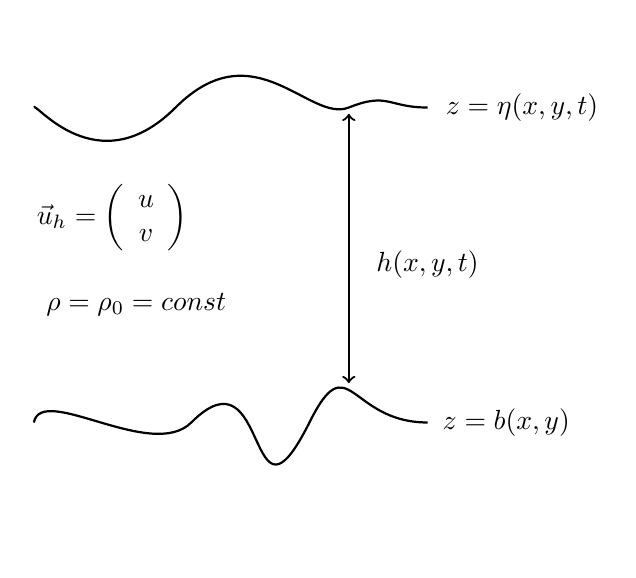
\begin{tikzpicture}
            \draw[thick] (0,0) .. controls +(0.1,0.5) and +(-0.5,-0.5) .. (2,0) .. controls +(1,1) and +(-0.8,-1.6) .. (3.5,0) .. controls +(0.5,1) and +(-1,0) .. (5,0);
            \node[] at (6,0) {$z=b(x,y)$};
            \draw[thick] (0,4) .. controls +(0,0.1) and +(-1,-1) .. (1.8,4) .. controls +(1,1) and +(-0.5,-0.2) .. (4,4) .. controls +(0.5,0.2) and +(-0.5,0) .. (5,4);
            \node[] at (6.2,4) {$z=\eta(x,y,t)$};
            \draw[thick,<->] (4,3.92) -- (4,0.5);
            \node[] at (5,2) {$h(x,y,t)$};
            \node[] at (1.3,1.5) {$\rho=\rho_0=const$};
            \node[] at (1,2.6) {$\vec{u}_h=\left( \begin{array}{c}u\\v\end{array} \right)$};
        \end{tikzpicture}
        \caption{The Shallow Water System}
    \end{figure}
    \end{minipage}
\end{fact}

We now aim to derive these equations from three primitive (approximate) equations: the horizontal momentum equation (\ref{Horizontal Approximate}), the vertical momentum equation (\ref{Vertical Approximate}), and mass conservation (\ref{Mass Conservation}). First, we neglect all vertical and horizontal forces $F_z$ and $\vec{F}_h$ (e.g. neglect friction) other than gravity and pressure gradient forces.

Second, we assume that the density is constant $\rho=\rho_0$ for all time and at all points. This immediately implies (from Equation \ref{Mass Conservation}) that the system must be incompressible, so we know that Equation \ref{Incompressibility} holds.

Third, we assume that the system is \textbf{shallow}: $H/L\ll 1$ where $H$ is the vertical lengthscale and $L$ is the horizontal lengthscale. If we non-dimensionalise \ref{Incompressibility}, we derive that the vertical velocity scale $W$ is much smaller than the horizontal velocity scale $U$: $W\ll U$:
\begin{align*}
    \vec{\nabla}\cdot\vec{u}=0\\
    \underbrace{\vec{\nabla}_h\cdot\vec{u}_h}_{U/L}+\underbrace{\frac{\partial w}{\partial z}}_{W/H}=0\\
    \therefore \frac{U}{L}\sim\frac{W}{H}\text{   }\therefore
    \frac{W}{U}\sim\frac{H}{L}\\
    \therefore \boxed{W \ll U}
\end{align*}

We take this as justification for our fourth assumption: that vertical acceleration and advection is small compared to gravity and pressure gradient forces. As such, the system is in approximately in \hyperref[Hydrostatic GFD]{Hydrostatic Balance} (we have simplified Equation \ref{Vertical Approximate} here). Importantly, though, we do \textit{not} assume that the vertical acceleration/advection is $0$ everywhere. We simply assume that they are much smaller than vertical pressure gradients and gravity.

This allows us to integrate the hydrostatic relation from some reference height $\eta$ (the height of the surface) and pressure $p_s$ (the pressure at the surface) to find that the following holds (refer to Equation \ref{Const Density Hydrostatic} to see the derivation).
\begin{align*}
    p(x,y,z,t)=\rho g(\eta(x,y,t)-z)+p_s(x,y,t)
\end{align*}

Fifth, we assume that the fluid above the layer of fluid under consideration has a much lower viscocity than the current layer or that it is much less dense than the other positions. This allows us to assume that $\vec{\nabla}_hp_s\ll \vec{\nabla}_h\eta$, and that therefore $\vec{\nabla}_h p \approx \rho_0 g \vec{\nabla}_h \eta$. As such, Equation \ref{Horizontal Approximate} becomes the following:
\begin{align*}
    \frac{D\vec{u}_h}{Dt}+f\vec{k}\times\vec{u}_h=g\vec{\nabla}_h\eta
\end{align*}

Notice that everything on the right hand side has no dependence on $z$. However, it must hold for each all $z$ within the layer, therefore, we can conclude that $\vec{u}_h$ cannot depend on $z$ either.\footnote{
    If it did, then the $f\vec{k}\times\vec{u}_h$ term would depend on $z$ and so left hand side would depend on $z$. Depending on $z$ implies that its value would change depending on $z$, but the right hand side cannot change its value depending on $z$, and so the equation would not hold for some $z$.
} Therefore, we can neglect the vertical advection term in the material derivative:
\begin{align*}
    \frac{D}{Dt}=\frac{\partial}{\partial t}+u\frac{\partial}{\partial x}
    +v\frac{\partial}{\partial y}+\bcancel{w\frac{\partial}{\partial z}}
\end{align*}

This allows us to derive Equation \ref{SW mom}, which is an approximation of the horizontal momentum equation (\ref{Horizontal Approximate}):
\begin{align*}
    \boxed{\frac{D_h\vec{u}_h}{Dt}+f\vec{k}\times\vec{u}_h=g\vec{\nabla}_h\eta}
\end{align*}
where $\frac{D_h}{Dt}=\frac{\partial}{\partial t}+u\frac{\partial}{\partial x}+v\frac{\partial}{\partial y}$ is the horizontal material derivative.

The interpretation is as follows: this is just horizontal momentum balance, where the horizontal acceleration is set by the coriolis force and the pressure gradient force, and no other forces. The pressure gradient force only depends on the height of the surface of the fluid, and the height affects the pressure through the hydrostatic relation.

Let us now turn to Mass Conservation Equation \ref{Mass Conservation}. We already derived from the $\rho=\rho_0=const$ assumption that the system must be incompressible, so the following holds:
\begin{align*}
    \vec{\nabla}\cdot\vec{u}=\vec{\nabla}_h\cdot\vec{u}_h+\frac{\partial w}{\partial z}=0
\end{align*}

Let us integrate this equation with respect to $z$ from $z=b(x,y)$ to $z=\eta(x,y,t)$ and recall first that $\vec{u}_h$ is not a function of $z$ and second that we assumed that $w$ was much smaller than $u,v$, not that $w=0$. This allows us to derive the following:
\begin{align*}
    \int_{b}^{\eta} 0 \,dz &= \int_{b}^{\eta} \vec{\nabla}_h\cdot\vec{u}_h+\frac{\partial w}{\partial z}\, dz\\
    0&=h(x,y,t)\vec{\nabla}_h\cdot\vec{u}_h+\left[ w \right]_b^\eta\\
    &=h\,\vec{\nabla}_h\cdot\vec{u}_h + w(z=\eta)-w(z=b)
\end{align*}
\begin{align*}
    \therefore \boxed{0 = h\,\vec{\nabla}_h\cdot\vec{u}_h + w(z=\eta)-w(z=b)}
\end{align*}

Now it turns out (and this is justified by some fluid mechanical boundary conditions) that $w(z=\eta)=\frac{D_h \eta}{Dt}$ and $w(z=b)=\frac{D_h b}{Dt}$. The interpretation is as follows: the vertical velocity at an interface must be exactly equal to the change in interface height/depth following a fluid parcel, because if this weren't the case, we would get a fluid parcel phasing through the ground (as is the case at the bottom where $z=b$) or the fluid parcel is exactly what sets the change in the interface depth (as is the case at the top where $z=\eta$).

As such:
\begin{align*}
    w(z=\eta)-w(z=b)&=\frac{D_h \eta}{Dt}-\frac{D_h b}{Dt}\\
    &=\frac{D_h h}{Dt}\\
    &=\frac{\partial h}{\partial t}+ \vec{u}_h\cdot\vec{\nabla}_hh
\end{align*}

Therefore, we get that:
\begin{align*}
    0&=h\,\vec{\nabla}_h\cdot\vec{u}_h + w(z=\eta)-w(z=b)\\
    &=h\,\vec{\nabla}_h\cdot\vec{u}_h+\frac{\partial h}{\partial t}+ \vec{u}_h\cdot\vec{\nabla}_hh\\
    0&=\frac{\partial h}{\partial t}+\vec{\nabla}_h\cdot(h\vec{u}_h)
\end{align*}

We have derived Equation \ref{SW mass}. The interpretation for this equation is as follows: the height of a fluid can change, but it is constrained by the velocity of the fluid becauce the fluid is incompressible. If the height increases at some point, there must be more fluid flowing into that point than out of it, but since the fluid cannot compress, the height of the layer must increase.

We have derived all the equations of motion for the Shallow Water System, but the crux of the issue is whether or not this is a faithful representation of time-dependent geophysical fluid dynamics. Sadly, the details are quite complicated, and I'm not sure if I'll even get to them. If I do, they are at the end of this chapter in Section \ref{SW Justification}.

For now, just take this as granted, and let us start analysing this system.

\section{Energetics}

Let us first consider the energy in the shallow water system, which the sum of the kinetic energy and the (gravitational) potential energy. Again, we would prefer to work in intensive variables, so we find these per unit area.

The kinetic energy per unit area is as follows:
\begin{align*}
    KE = \frac{1}{2}\underbrace{\rho_0\,V}_{m}\,u^2/A\\
    =\frac{1}{2}\rho_0\,A\,h/A\,u^2\\
    \therefore\BOX{KE = \frac{1}{2}\rho_0\,h\,u^2}
\end{align*}
The idea is simple: it's just the kinetic energy divided by the unit area.

The potential energy per unit area is a little bit more complicated. To find this, we need to consider all the fluid parcels from $z=b$ to $z=\eta$ and sum the potential energy of all the fluid parcels.

Let us first consider a fluid parcel at height $z$ with some height $dz$ and width $A$ (therefore, it has a volume equal to $A\,dz$ and mass equal to $\rho_0\,A\,dz$). The potential energy of \textit{this} parcel ($dPE$) is as follows:
\begin{align*}
    dPE=\underbrace{\rho_0\,a\,dz}_{m}g\,z
\end{align*}
We have to sum this over all the fluid parcels from $z=b$ to $z=\eta$ so our total potential energy per unit area $PE$ is as follows:
\begin{align*}
    PE &= \int_{z=b}^{z=\eta}dPE/A\\
    &= \int_{z=b}^{z=\eta}\underbrace{\rho_0\,A\,dz}_{m}g\,z/A\\
    &= \rho_0\,g\left[ \frac{1}{2}z^2 \right]_b^\eta\\
    &= \frac{1}{2}\rho_0\,g\left( \eta^2-b^2 \right)
\end{align*}

Now the final fiddly thing we have to do is to say that we don't actually care about the 

\section{Potential Vorticity}

\section{Waves}

\subsection{A Quick Primer on Waves}

In the previous section, we derived geostrophic balance and  hydrostatic balance. 

However, the Earth is never in perfect balance, and small perturbations will occur, either because we have built a wind farm, or the sun is radiating differently, or because freshwater is being injected into certain areas in the oceans.

We analyse how systems respond to these perturbations by looking for wave-like solutions: we plug in a solution that is proportional to $\exp(i(\vec{k}\cdot\vec{x}-\omega t))$, where $\vec{k}=(k_x,k_y,k_z)^T\in\mathbb{R}^3$ is the angular wavevector (the vector analogue of the wavenumber – refer to Section \ref{F, W, W} if you've forgotton what a wavenumber is) and $\omega$ is the angular frequency.

The justification for plugging in this somewhat convoluted function is as follows. We want a function that is simple enough such that the solution is easy to interpret. However, we also want a function complicated enough such that it can encode certain spatial and time dependencies. This is why we pick the exponential function, which is simple, which depends on a linear sum of space and time, which.

In practice, after plugging in these equations, we will find that $\vec{k}$ and $\omega$ are constrained by the equations of motion such that:
\begin{align*}
    \omega=\omega(\vec{k})
\end{align*}

In other words, the frequency with which the perturbation oscillates is set by the spatial scale (or vice versa). This will give us valuable information regarding how these waves propogate.

We will find that the peaks and troughs in the wave will propogate with a \textbf{phase velocity} denoted by $\vec{c}_p$, where the $i$th component $[\vec{c}_p]_i$ is found as follows:
\begin{align}
    \label{Phase Velocity}
    \BOX{[\vec{c}_p]_i=\frac{\omega}{[\vec{k}]_i}}
\end{align}

We will also find that a wave-packet will propogate with a \textbf{group velocity} denoted by $\vec{c}_g$, where the $i$th component $[\vec{c}_g]_i$ is found as follows:
\begin{align}
    \label{Group Velocity}
    \BOX{[\vec{c}_g]_i=\frac{\partial\omega}{\partial [\vec{k}]_i}}
\end{align}
For example, in the $x$ direction, the \textbf{group} and \textbf{phase velocities} are found as follows:
\begin{align*}
    [\vec{c}_p]_x=\frac{\omega}{k_x}\\
    [\vec{c}_g]_x=\frac{\partial\omega}{\partial k_x}
\end{align*}

This is a slightly confusing distinction, as you've most likely only encountered non-dispersive waves in the past, and non-dispersive waves are waves such that the phase velocity is equal to the group velocity ($\vec{c}_g=\vec{c}_p$). Since I can't insert any animations into these pdf notes, I'd highly recommend clicking on \href{https://resource.isvr.soton.ac.uk/spcg/tutorial/tutorial/Tutorial_files/Web-further-dispersive.htm}{this} website on dispersive waves. I'd especially pay attention to the little animations.

Now that you've thoroughly read that resource, we can interpret what this means in our context. Suppose that the pressure perturbation is proportional to $\exp(i(\vec{k}\cdot\vec{x}-\omega t))$ where $\omega=\omega(\vec{k})$ such that $\vec{c}_p=\vec{c}_p(\vec{k})$ and $\vec{c}_g=\vec{c}_g(\vec{k})$. Peaks and troughs propagate with a velocity set by the \textbf{phase velocity} $\vec{c}_p=\vec{c}_p(\vec{k})$, so areas of low or high pressure (i.e., cyclones and anti-cyclones in mid-/high-latitudes) propogate at the velocity $\vec{c}_p$. Meanwhile, the amplitude of this low or high pressure perturbation propagates with a velocity set by the \textbf{group velocity} $\vec{c}_g=\vec{c}_g(\vec{k})$. You saw that, in general, this means that the energy propagates with the \textbf{group velocity}, \textit{not} the \textbf{phase velocity}.

\subsection{Poincaré Waves}

We first linearise the Shallow Water Equations about a state of rest $\vec{U}=0$ and layer thickness $H$. For simplicity we assume a flat bed $b=-H=const$. This is the first time we linearise in this course, so I will go through this a bit more carefully.

First, we write our variables as a sum of the unvarying quantity and the small perturbation:

\begin{align*}
    \vec{u}=\vec{U}+\vec{u}'\\
    h = H + h'\\
    \eta = N + \eta'\\
\end{align*}

\noindent where $|\vec{U}|\gg \vec{u}'$, $H\gg h'$, and $N\gg \eta'$. 

Second, we substitute these equations into the shallow water equations, then eliminate terms that are not zeroth or first order in the primed quantites. For example, for Equation \ref{SW height}:

\begin{align*}
    \frac{\partial}{\partial t}\left( H+h' \right)+\vec{\nabla}\cdot \left( (H+h')(\vec{U}+\vec{u}') \right)=0\\
    \frac{\partial}{\partial t}\left( H+h' \right)+\vec{\nabla}\cdot \left( H\vec{U}+H\vec{u}'+h'\vec{U}+\bcancel{h'\vec{u}'} \right)=0\\
\end{align*}

T


\subsection{Kelvin Waves}

\subsection{Rossby Waves}

\section{Justifying the Shallow Water System}\label{SW Justification}

\chapter{3D Systems}

\section{Gravity Waves}

\subsection{The Boussinesq Approximation}

\section{Quasi-Geostrophic Theory}

\section{Quasi-Geostrophic Rossby Waves}

\section{Instabilities and Geostrophic Turbulence}

\chapter{Ocean Circulation}

As already touched upon, the oceans, while similar to the atmosphere in the sense that it is a fluid affected by gravity (and so stratification) and rotation (and so coriolis), differs dynamically due to a few facts.

\begin{enumerate}
    \item Equation of state: $g'$ is much smaller, so $L_d$ is much smaller
    \item Rossby number
    \item External forcing
    \item Bathymetry
\end{enumerate}

We'll be exploring some effects of external forcing \ref{Ekman Transport} and the small rossby number \ref{Sverdrup Balance}.

\section{Ekman Transport}\label{Ekman Transport}

Assume $Ro\ll1$ so we can 

\begin{align}
    f\vec{k}\times\vec{u}=\frac{1}{\rho}
\end{align}

\section{Sverdrup Balance}\label{Sverdrup Balance}

\section{Stommel Box Model}\label{MOC}